In \cite{Teachlet} wird die effektive Berechnung der Masse Matrix mit einem Vektor multipliziert, vorgestellt. Diese Methodik sollten wir uns kurz vor Augen führen und daraufaufbauend um einige eigene Gedanken erweitern um sie für unsere Anwendung zugänglich zu machen.
Das Ziel dieses Unterkapitels ist es die Tensorstruktur für die Massematrix und der Laplace Bilinearform herzuleiten und für die Berechnung der Pseudoinversen zu nutzen. 

\subsubsection{Tensorstruktur der Elementmassenmatrix}
Es sei $T$ die Referenzzelle für Rechtecke und $\varphi^{2D}_i(\bold{x})$ zweidimensionale reelle Basisfunktion des diskreten Raumes $V_n$ mit $\bold{x}=(x,y)$ .
\begin{equation} \label{eq:mass}
M_{ik} = \int\limits_{T} \varphi^{2D}_i (\bold{x}) \, \varphi^{2D}_j (\bold{x}) \, d\bold{x}
\end{equation}

Die Basisfunktionen haben eine Tensorstruktur, die wie folgt aussieht
\begin{equation} \label{eq:tensor}
\varphi^{`2D}_i(\bold{x})=\varphi^{2D}_{i_1+(N+1)i_2}(x,y)=\varphi^{1D}_{i_1}(x)\varphi^{1D}_{i_2}(y),
\end{equation}

wobei $\varphi^{`2D}$ eine eindimensionale reelle Basisfunktion ist.

Wir werden eine lexikographische Ordnung der Freiheitsgrade benutzen. Die Reichweite von $\, \, i_1 $ und $ i_2 \, $ reicht von $1$ bis $N$. Das heißt der Index $i$ geht von $1$ bis $N_p=(N+1)^2$. In Abbildung (\ref{fig:lexi}) sehen Sie ein Beispiel für $N=3$.

\begin{figure}[ht] 
	\centering
  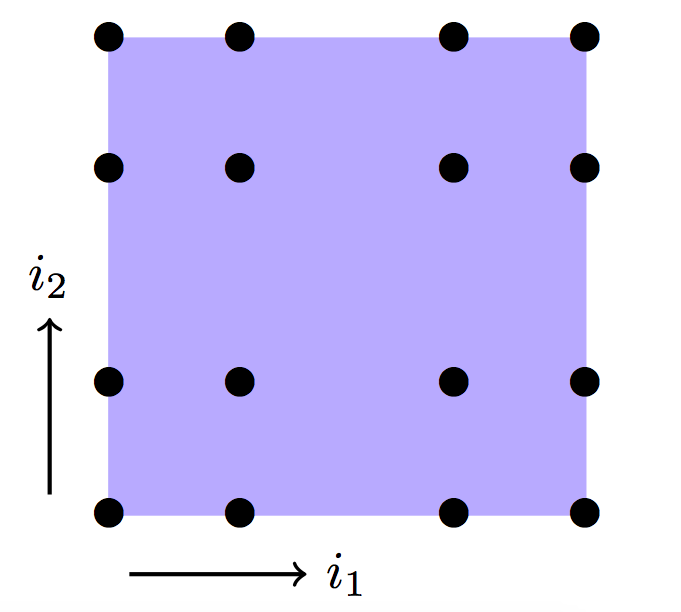
\includegraphics[width=0.3\textwidth]{lexi.png}
	\caption{ \cite[3]{Teachlet}}
	\label{fig:lexi}
\end{figure}

Wir wollen für die Berechnung der Integrale in (\ref{eq:mass}) die Gauss Quadratur benutzen.
Es seien $\bold{x}_q=(x_{q1},x_{q2})$ die Stützstellen und $\bold{w}_q=w_{q1}w_{q2}$ die Gewichte. Die Gleichung (\ref{eq:mass}) kann approximiert werden durch

\begin{equation} \label{eq:massapprox}
\begin{aligned}
M_{ij} &= \int\limits_{T} \varphi_i (\bold{x}) \, \varphi_j (\bold{x}) \, d\bold{x} \\
&\approx  \sum\limits_{q=1}^Q \bold{w}_q \, \, \varphi_i (\bold{x}_q) \, \varphi_j (\bold{x}_q) \\
&= \sum\limits_{q_1=1}^{Q_{1D}} \sum\limits_{q_2=1}^{Q_{1D}} \varphi_{i_1}(x_{q1}) \varphi_{i_2}(x_{q2}) \varphi_{j_1}(x_{q1}) \varphi_{j_2}(x_{q2}) \, w_{q1} w_{q2} \\ 
&= \sum\limits_{q_1=1}^{Q_{1D}} w_{q1} \varphi_{i_1}(x_{q1}) \varphi_{j_1}(x_{q1}) \sum\limits_{q_2=1}^{Q_{1D}} w_{q2} \varphi_{i_2}(x_{q2}) \varphi_{j_2}(x_{q2}) \, . 
\end{aligned}
\end{equation}

Wir wählen die Anzahl der Quadraturpunkte $Q_{1D}$ per Dimension so, dass wir exakt integrieren. Wir wählen $Q_{1D}$ gleich der Anzahl der Basisfunktionen $N$, da wir mit der Gauss Quadratur mit $N+1$ Stützstellen bis $2N$ exakt integrieren und der höchste Grad bei uns $2N$ ist.

Wir definieren uns eine Matrix durch $\mathcal{N}_{iq}=\varphi_i(x_q)$ und weiterhin die Matrix $\mathcal{W}_{ii}=\bold{w}_i$, die in der Diagonalen die Quadraturgewichte hat und sonst Nullen. Damit können wir nun die Massematrix schreiben als
\begin{equation}
M = \mathcal{N} \mathcal{W} \mathcal{N}^T
\end{equation}

In $\mathcal{N}$ sind die Elemente an Stützstellen evaluierte zweidimensionale Basisfunktionen. Wir können dies aber weiter aufspalten in eindimensionale Basisfunktionen, dank der Tensorstruktur der Basisfunktionen, und dadurch eine Effizienzsteigerung erzielen bei der Berechnung des Matrix-Vektor Produkts mit der Elementmassenmatrix.

Wir fangen damit an, die Matrix $\mathcal{N}$ in ein Tensorprodukt aufzuspalten. 
\begin{equation} \label{eq:onedim}
\mathcal{N} = \mathcal{N}^{1D} \otimes \mathcal{N}^{1D}
\end{equation}

Die Matrix $\mathcal{N}^{1D}$ ist nun äquivalent definiert wie $\mathcal{N}$ bloß mit eindimensionalen Basisfunktionen. Ausgeschrieben sieht die Gleichung (\ref{eq:onedim}) wie folgt aus:

\begin{equation*}
\begin{bmatrix}
\varphi^{2D}_1(\bm{x}_1) & \hdots & \varphi^{2D}_N(\bm{x}_1) \\
\vdots & \ddots & \vdots \\
\varphi^{2D}_1(\bm{x}_Q) & \hdots & \varphi^{2D}_N(\bm{x}_Q)
\end{bmatrix}
=
\begin{bmatrix}
\varphi^{1D}_1(x_1) & \hdots & \varphi^{1D}_n(x_1) \\
\vdots & \ddots & \vdots \\
\varphi^{1D}_1(x_{Q_{1D}}) & \hdots & \varphi^{1D}_n(x_{Q_{1D}})
\end{bmatrix}
\otimes
\begin{bmatrix}
\varphi^{1D}_1(x_1) & \hdots & \varphi^{1D}_n(x_1) \\
\vdots & \ddots & \vdots \\
\varphi^{1D}_1(x_{Q_{1D}}) & \hdots & \varphi^{1D}_n(x_{Q_{1D}})
\end{bmatrix}
\end{equation*}.

Wir nutzen absofort $Q_{1D}=N+1$ und $Q=(N+1)^2$, da wie wir oben bereits argumentiert haben, damit exakt integrieren können.
Wir erinnern uns $M=\mathcal{N} \mathcal{W} \mathcal{N}^T$. Da $\mathcal{W}$ eine Diagonalmatrix ist, ist es naheliegend diese Multiplikation bereits durchzuführen. Definiere $\mathcal{W}_{N}=\mathcal{N} \mathcal{W}$ und die Spaltung von $\mathcal{W}_N$ kann im nächsten Schritt hergeleitet werden.

\begin{equation} \label{eq:weight}
\mathcal{W}_N = \mathcal{W}_N^{1D} \otimes \mathcal{W}_N^{1D}
\end{equation}

Genauer

\begin{equation*}
\begin{bmatrix}
\mathcal{N}_{11} \bold{w}_1 & \hdots & \mathcal{N}_{1N} \bold{w_N} \\
\vdots & \ddots & \vdots \\
\mathcal{N}_{N1} \bold{w}_1 & \hdots & \mathcal{N}_{NN} \bold{w_N}
\end{bmatrix}
= 
\begin{bmatrix}
\mathcal{N}_{11}^{1D} w_1 & \hdots & \mathcal{N}_{1N}^{1D} w_N \\
\vdots & \ddots & \vdots \\
\mathcal{N}_{N1}^{1D} w_N & \hdots & \mathcal{N}_{NN}^{1D} w_N
\end{bmatrix}
\otimes
\begin{bmatrix}
\mathcal{N}_{11}^{1D} w_1 & \hdots & \mathcal{N}_{1N}^{1D} w_N \\
\vdots & \ddots & \vdots \\
\mathcal{N}_{N1}^{1D} w_1 & \hdots & \mathcal{N}_{NN}^{1D}w_N
\end{bmatrix}
\end{equation*}.

Damit können wir folgende Umformulierung bereits vornehmen
\begin{equation}
M= \mathcal{N} \mathcal{W} \mathcal{N}^T= \mathcal{W}_N \mathcal{N}^T =  [\mathcal{W}_N^{1D} \otimes \mathcal{W}_N^{1D}]  [\mathcal{N}^{1D} \otimes \mathcal{N}^{1D}]^T.
\end{equation}

Mit Lemma (\ref{lemma:transpose}) folgt
\begin{equation*}
[\mathcal{W}_N^{1D} \otimes \mathcal{W}_N^{1D}] [\mathcal{N}^{1D} \otimes \mathcal{N}^{1D}]^T=
[\mathcal{W}_N^{1D} \otimes \mathcal{W}_N^{1D}]  [(\mathcal{N}^{1D})^T \otimes (\mathcal{N}^{1D})^T].
\end{equation*}

Dann nutzen wir Lemma (\ref{lemma:prod}) und erhalten
\begin{equation}
 [\mathcal{W}_N^{1D} \otimes \mathcal{W}_N^{1D}]  [(\mathcal{N}^{1D})^T \otimes (\mathcal{N}_{1D})^T]= [\mathcal{W}_N^{1D} (\mathcal{N}^{1D})^T] \otimes [\mathcal{W}_N^{1D} (\mathcal{N}_{1D})^T].
\end{equation}

\newpage
\subsubsection{Tensorstruktur der Elementsteifigkeitsmatrix der Laplace Bilinearform}
Die Formel, leicht geändert, kann benutzt werden um andere Bilinearformen auszudrücken wie die Laplace Bilinearform. Es sei die Elementsteifigkeitsmatrix der Laplace Bilinearform elementweise gegeben durch

\begin{equation}
V_{ij} = \int\limits_{T} \nabla \varphi_i(\bold{x}) \, \nabla \varphi_j(\bold{x})  d \bold{x}=\int\limits_{T}( \partial_{x_1}  \varphi_i(\bold{x})  \partial_{x_1} \varphi_j(\bold{x})) + ( \partial_{x_2} \varphi_i(\bold{x})  \partial_{x_2} \varphi_j(\bold{x})) \, d\bold{x}.
\end{equation}

Wir nutzen die Linearität des Integrals.
\begin{equation}
\begin{aligned}
V_{ij} &= \int\limits_{T}( \partial_{x_1}  \varphi_i(\bold{x})  \partial_{x_1} \varphi_j(\bold{x})) + ( \partial_{x_2} \varphi_i(\bold{x})  \partial_{x_2} \varphi_j(\bold{x})) \, d\bold{x} \\ &= \int\limits_{T} \partial_{x_1}  \varphi_i(\bold{x})  \partial_{x_1} \varphi_j(\bold{x}) d\bold{x} + \int\limits_{T}  \partial_{x_2} \varphi_i(\bold{x})  \partial_{x_2} \varphi_j(\bold{x}) \, d\bold{x}
\end{aligned}
\end{equation}

Für die Integrale verwenden wir wieder die Gauss Quadratur.. Es seien $\bold{x}_q=(x_{q1},x_{q2})$ die Stützstellen und $\bold{w}_q=w_{q1}w_{q2}$ die Gewichte, dann folgt für die obere Gleichung

\begin{equation}
\begin{aligned}
V_{ij}  = \underbrace{\sum\limits_{q=1}^{(N+1)^2} \bold{w}_q \partial_{x_1}  \varphi_i(\bold{x}_q)  \partial_{x_1} \varphi_j (\bold{x}_q)}_{K_1} + \underbrace{\sum\limits_{q=1}^{(N+1)^2} \bold{w}_q  \partial_{x_2} \varphi_i(\bold{x}_q)  \partial_{x_2} \varphi_j(\bold{x}_q)}_{K_2} \, .
\end{aligned}
\end{equation}

Wir können eine große Ähnlichkeit mit der Struktur der Massematrix in (\ref{eq:massapprox}), wenn wir uns jeweils nur $K_1$ und $K_2$ seperat anschauen. Jetzt gilt es die Tensorstruktur der Ansatzfunktionen auszunutzen. Dafür betrachten wir $K_1$.
\begin{equation}
\begin{aligned}
K_1 &=\sum\limits_{q=1}^{(N+1)^2} \bold{w}_q \partial_{x_1}  \varphi_i(\bold{x}_q)  \partial_{x_1} \varphi_j (\bold{x}_q) \\ &= \sum\limits_{q_1=1}^{N} \sum\limits_{q_2=1}^{N} w_{q1}w_{q2} \partial_{x_1}  \varphi_{i1}(x_{q1})\varphi_{i2}(x_{q2})  \partial_{x_1} \varphi_{j1} (x_{q1})\varphi_{j2} (x_{q2}) \\
&=  \sum\limits_{q_1=1}^{N} \sum\limits_{q_2=1}^{N} w_{q1}w_{q2} \varphi'_{i1}(x_{q1})\varphi_{i2}(x_{q2})  \varphi'_{j1} (x_{q1})\varphi_{j2} (x_{q2}) \\ 
&= \sum\limits_{q_1=1}^{N} w_{q1} \varphi'_{i1}(x_{q1}) \varphi'_{j1} (x_{q1}) \sum\limits_{q_2=1}^{N} w_{q2} \varphi_{i2}(x_{q2})  \varphi_{j2} (x_{q2}) 
\end{aligned}
\end{equation}

Man kann die Ähnlichkeit mit der Gleichung (\ref{eq:massapprox}) erkennen. Wir sehen, dass wir in einer Dimension nun aber die evaluierten Ableitungen der Basisfunktionen und in die andere Dimension die evaluierten Basisfunktionen haben.
Wir definieren uns zwei Matrizen $\widehat{\mathcal{W}}^{1D}_N$ und $\widehat{\mathcal{N}}^{1D}$ die ähnlich sind zu $\mathcal{W}^{1D}$ und $\mathcal{N}^{1D}$ mit dem Unterschied, dass diese Matrizen nicht die Ansatzfunktionen evaluieren sondern deren Ableitung.

\begin{equation}
\widehat{\mathcal{N}}^{1D} = 
\begin{bmatrix}
\varphi'^{ \, 1D}_1(x_1) & \hdots &  \varphi'^{ \, 1D}_n(x_1) \\
\vdots & \ddots & \vdots \\
\varphi'^{ \, 1D}_1(x_N)& \hdots & \varphi'^{ \, 1D}_n(x_N)
\end{bmatrix}
\end{equation}

Analog definieren uns $\widehat{\mathcal{W}}^{1D}_N$.
Dann folgt mit analoger Umformung wie bei der Massematrix

\begin{equation}
K_1 = K_2^T = (\widehat{\mathcal{W}}_N^{1D} (\widehat{\mathcal{N}}^{1D})^T) \otimes (\mathcal{W}_N^{1D} (\mathcal{N}^{1D})^T).
\end{equation}


Insgesamt kann man die Elemensteifigkeitsmatrix für die Laplace Bilinearform darstellen als
\begin{equation}
V =[\widehat{\mathcal{W}}_N^{1D} (\widehat{\mathcal{N}}^{1D})^T] \otimes [\mathcal{W}_N^{1D} (\mathcal{N}^{1D})^T] + ([\widehat{\mathcal{W}}_N^{1D} (\widehat{\mathcal{N}}^{1D})^T] \otimes [\mathcal{W}_N^{1D} (\mathcal{N}^{1D})^T])^T.
\end{equation}


\subsubsection{Pseudoinverse}

Die Pseudoinversen für die Elementsteifigkeitsmatrix der Massematrix $M$ und der Laplace Bilinearform $V$ gilt es jetzt herzuleiten. Dank unserer Vorarbeit und unserem Vorwissen zum Kronecker Produkt, ist es möglich, dies problemlos zu machen.

Rekapituliere die Tensorstruktur für die Massematrix
\begin{equation}
M =  ([\mathcal{W}_N^{1D} (\mathcal{N}^{1D})^T] \otimes [\mathcal{W}_N^{1D} (\mathcal{N}_{1D})^T].
\end{equation}
Nun wollen wir die Pseudoinverse herleiten
\begin{equation}
M^+=  [(\mathcal{W}_N^{1D} (\mathcal{N}^{1D})^T] \otimes [\mathcal{W}_N^{1D} (\mathcal{N}_{1D})^T)]^+ .
\end{equation}

Wir nutzen Lemma (\ref{lemma:inverse}) und erhalten
\begin{equation}
[(\mathcal{W}_N^{1D} (\mathcal{N}^{1D})^T] \otimes [\mathcal{W}_N^{1D} (\mathcal{N}_{1D})^T])^+ =  [\mathcal{W}_N^{1D} (\mathcal{N}^{1D})^T]^+ \otimes [\mathcal{W}_N^{1D} (\mathcal{N}_{1D})^T]^+.
\end{equation}

Hier können wir nun eine Singulärwertzerlegung oder den Gauß Algorithmus. zum berechnen der korrekten Inversen, verwenden. Dies geht, weil  $\mathcal{N}^{1D}$ und $\mathcal{W}_N^{1D}$ invertierbar sind.  Warum das Ganze? Wir hätten auch die Inverse von der Massematrix berechnen können. Der Unterschied ist, dass wir statt der Inversen einer Matrix der Größe $N^2 \times N^2$ berechnen, berechnen wir die Inverse einer Matrix der Größe $N \times N$.

Für die Laplace Bilinearform können wir dies leider nicht so einfach machen. Das Problem ist die Addition, die uns das ganze stark erschwert. Je nach Basis, kann man das Problem vereinfachen. Man könnte beispielsweise die Lagrange Basis nehmen mit geeigneten Stützstellen und würde für $\mathcal{N}^{1D}$ und $\mathcal{W}_N^{1D}$ Diagonalmatrizen bekommen.

Wir brauchen ein Hilfswerkzeug, dass uns mit dem Inversen von der Summe von Matrizen hilft. 

Was uns letztlich interessiert ist die Auswertung der Pseudoinversen an einem Vektor $u$ also $M^+ u$ und $V^+ u$. Wie wir dies effizient ausrechnen und welche Komplexität uns erwartet, sehen wir in Kapitel 4.

